\section{Vergleich}
Für die App-Programmierung stehen viele verschiedene Rahmenwerke bereits zur Verfügung.
Dieser Abschnitt beschäftigt sich mit dem Vergleich der einzelnen Möglichkeiten, sowie einer endgültigen Auswahl eines der Rahmenwerke zur Verwendung im Diplomprojekt.

\paragraph{Microsoft Xamarin}
ist ein Rahmenwerk, mit dem man Multiplattform-Applikationen für unter Anderem Android, iOS, UWP und noch viele weitere Plattformen erstellen kann.
Es basiert auf Microsofts \ac{dotnet} und dem Mono-Projekt, welches sich als Ziel gesetzt hat, das \ac{dotnet} auf andere Plattformen zu portieren.
Xamarin bietet mehrere Projekttypen an, darunter Xamarin.Android und Xamarin.iOS für native App-Entwicklung und Xamarin.Forms für großteils plattformunabhängige Entwicklung.
Eine Xamarin.Forms-Solution besteht daher aus drei Teilen: einem Portable/.NET-Standard-Projekt und je ein natives Xamarin-Projekt für jede Zielplattform.
Der Vorteil Xamarins ist, dass der Großteil des geschriebenen Codes im plattformunabhängigen Projekt bleibt und nur für wenige Funktionen auf native Programmierung zurückgegriffen wird, wie zum Beispiel für hardwarenahe Audio-Aufnahme.
Außerdem ist das Xamarin-Projekt Open Source, das bedeutet jeder kann den Quellcode betrachten und unter Umständen Verbesserungen vorbringen.

\paragraph{Apache Cordova}
ist ein Appentwicklungs-Rahmenwerk welches ursprünglich von der Firma Nitobi entwickelt wurde.
Im Jahr 2011 wurde Nitobi von Adobe aufgekauft und das Rahmenwerk wurde zu PhoneGap umgetauft.
Später wurde eine quelloffene Version unter dem ursprünglichen Namen veröffentlicht.
Apps werden mittels gängiger Webtechnologie, wie zum Beispiel JavaScript, CSS und Ähnlichen, entwickelt und realisiert, weshalb das Rahmenwerk alle gängigen Plattformen unterstützt.
Der Vorteil von Cordova liegt im enormen Support dieser Webtechnologien, jedoch sind Sprachen wie JavaScript nicht für Back-End-Programmierung geeignet.
Noch dazu kommt, dass an der HTL Anichstraße großteils die Programmierung nur in C und C\# gelehrt wird, welshalb die Entwicklung mit JavaScript nicht realistisch ist.

\paragraph{Andere}
Neben Apache Cordova existieren noch viele weitere Rahmenwerke, die wie Cordova auf Webtechnologie aufbauen, um so die Platformunabhängigkeit garantieren zu können. Allerdings bringen diese alle dieselben Probleme wie Cordova mit sich.

\section{Build-Umgebung}
Aufgrund obiger Aufstellung wurde Visual Studio 2019 der Firma Microsoft als Entwicklungsumgebung gewählt.
Visual Studio ist das offizielle Werkzeug für die Programmierung mit dem Xamarin-Rahmenwerk und die wahrscheinlich bestbekannte Entwicklungsumgebung überhaupt.
Die Community-Edition für Schüler und Private steht gratis zum Download zur Verfügung.
Diese beinhält alle wichtigen Entwicklungswerkzeuge wie zum Beispiel die automatische Code-Vervollständigung.
Für die Nutzung wird nach den ersten 30 Tagen ein Microsoft-Konto benötigt.\par
%versionsvergleich hier https://visualstudio.microsoft.com/vs/compare/

Visual Studio 2019 organisiert den Programmcode in sogenannten Solutions.
Am Beispiel einer Xamarin.Forms-Applikation lässt sich das sehr gut erläutern;
die Solution enthält auf oberster Ebene drei Projekte: das portable Projekt, das Android- und das iOS-Projekt.
Ein Projekt kann bereits für sich lauffähig oder nur Teil eines größeren Programms sein.\par

Visual Studio 2019 unterstützt viele verschiedene Einsatzbereiche, die bei der Installation ausgewählt werden müssen.
Eine volle Installation mit allen Funktionen und Projektarten ist zwar möglich, benötigt allerdings bis zu 210GB Speicherplatz des Systems.
Eine typische Xamarin-Installation benötigt zwischen 7GB und 10GB.
Für eine solche Installation muss im Visual Studio Installer das \enquote{Mobile development with .NET}-Paket ausgewählt und installiert werden.
\begin{figure}[H]
    \centering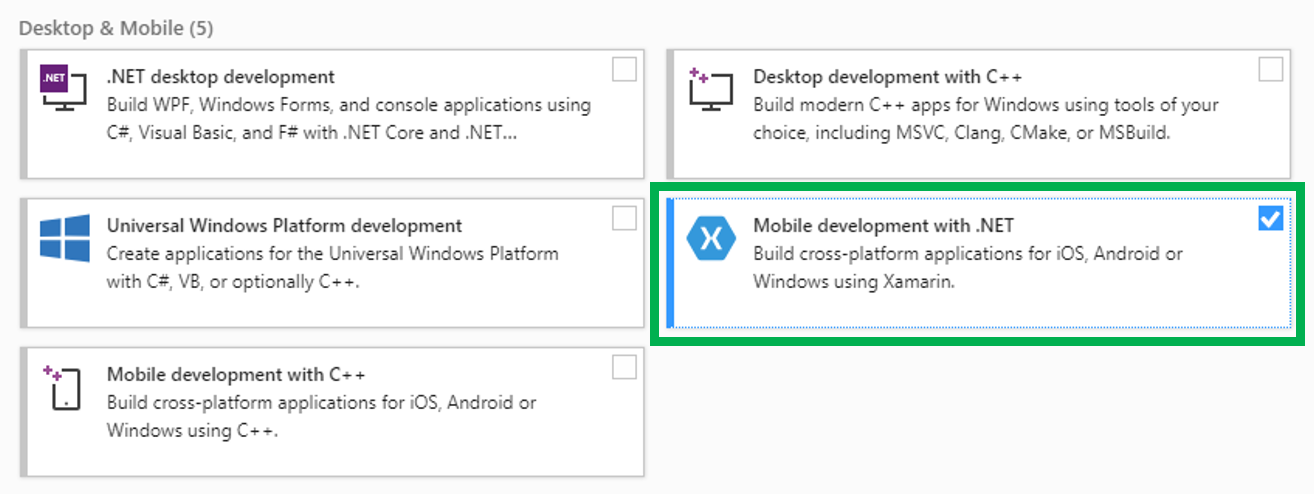
\includegraphics[width=0.9\linewidth]{images/auswahl_rahmenwerk/installation.png}    
    \caption{Auswahl des Xamarin-Rahmenwerks bei der Installation}
\end{figure}
Auf nähere Details der Installation von Visual Studio wird hier nicht eingegangen, diese können aber auf der Microsoft-Dokumentationsseite \cite[vgl.][]{msdoc-vs-install} nachgeschlagen werden.
%Betriebssystem, Hardwareanforderungen
%
\subsection{Installation Visual Studio} %nur wenn noch Text gebraucht wird
Die minimalen Hardware-, bzw. Software-Anforderungen können der \href{https://docs.microsoft.com/en-us/visualstudio/releases/2019/system-requirements}{Microsoft-Doku\-men\-tation des Visual Studio} entnommen werden:

\begin{table}[H]
    \centering\begin{tabulary}{0.9\linewidth}{|R|L|}
        \hline
        Unterstützte Betriebssysteme
        & - Windows 10, Version 1703 oder höher (LTSC und S werden nicht unterstützt)\\
        & - Windows Server 2019\\
        & - Windows Server 2016\\
        & - Windows 8.1 (mit Update 2919355)\\
        & - Windows Server 2012 R2 (mit Update 2919355)\\
        & - Windows 7 SP1 (mit neuesten Windows-Updates)\\
        \hline
        Hardware
        & - 1,8-GHz-Prozessor oder schneller; Quad-Core oder besser empfohlen\\
        & - 2 GB RAM; 8 GB RAM empfohlen\\
        & - Speicherplatz auf der Festplatte: Mindestens 800 MB, je nach installierten Features bis zu 210 GB des verfügbaren Speicherplatzes. Eine typische Installation erfordert 20–50 GB freien Speicherplatz.\\
        & - Festplattengeschwindigkeit: Zur Verbesserung der Leistung installieren Sie Windows und Visual Studio auf einem Festkörperlaufwerk (SSD).\\
        & - Grafikkarte, die eine Auflösung von mindestens 720p (1280 x 720) unterstützt. Visual Studio funktioniert am besten mit einer Auflösung von WXGA (1366 x 768) oder höher.\\
        \hline
    \end{tabulary}
    \caption{Soft- und Hardware-Anforderungen Visual Studio}    
\end{table}

%Quellenangabe!!
%Anforderungen für Android Emulator
% Der Android-Emulator hat zusätzliche Anforderungen, die über die grundlegenden Systemanforderungen für Android Studio hinausgehen, die im Folgenden beschrieben werden:

%     SDK-Tools 26.1.1 oder höher
%     64-Bit-Prozessor
%     Fenster: CPU mit UG-Unterstützung (uneingeschränkter Gast)
%     HAXM 6.2.1 oder höher (HAXM 7.2.0 oder höher empfohlen)

% Der Einsatz von Hardwarebeschleunigung stellt unter Windows und Linux zusätzliche Anforderungen:

%     Intel-Prozessor unter Windows oder Linux: Intel-Prozessor mit Unterstützung für Intel VT-x, Intel EM64T (Intel 64) und Execute Disable (XD)-Bit-Funktionalität
%     AMD-Prozessor unter Linux: AMD-Prozessor mit Unterstützung für AMD-V-Virtualisierung (AMD-V) und Supplemental Streaming SIMD Extensions 3 (SSSE3)
%     AMD-Prozessor unter Windows: Android Studio 3.2 oder höher und Windows 10. April 2018 oder höher für die Windows Hypervisor-Plattform (WHPX)

% Um mit Android 8.1 (API-Level 27) und höheren Systembildern arbeiten zu können, muss eine angeschlossene Webcam die Fähigkeit haben, 720p-Frames aufzunehmen.

%Vorsicht bei der Installation

Auf der oben genannten Website steht der Visual Studio 2019 Installer zum Download bereit.
Hier ist bereits die gewünschte Version, in diesem Fall die Community-Edition, auszuwählen.
\begin{figure}[H]
    \centering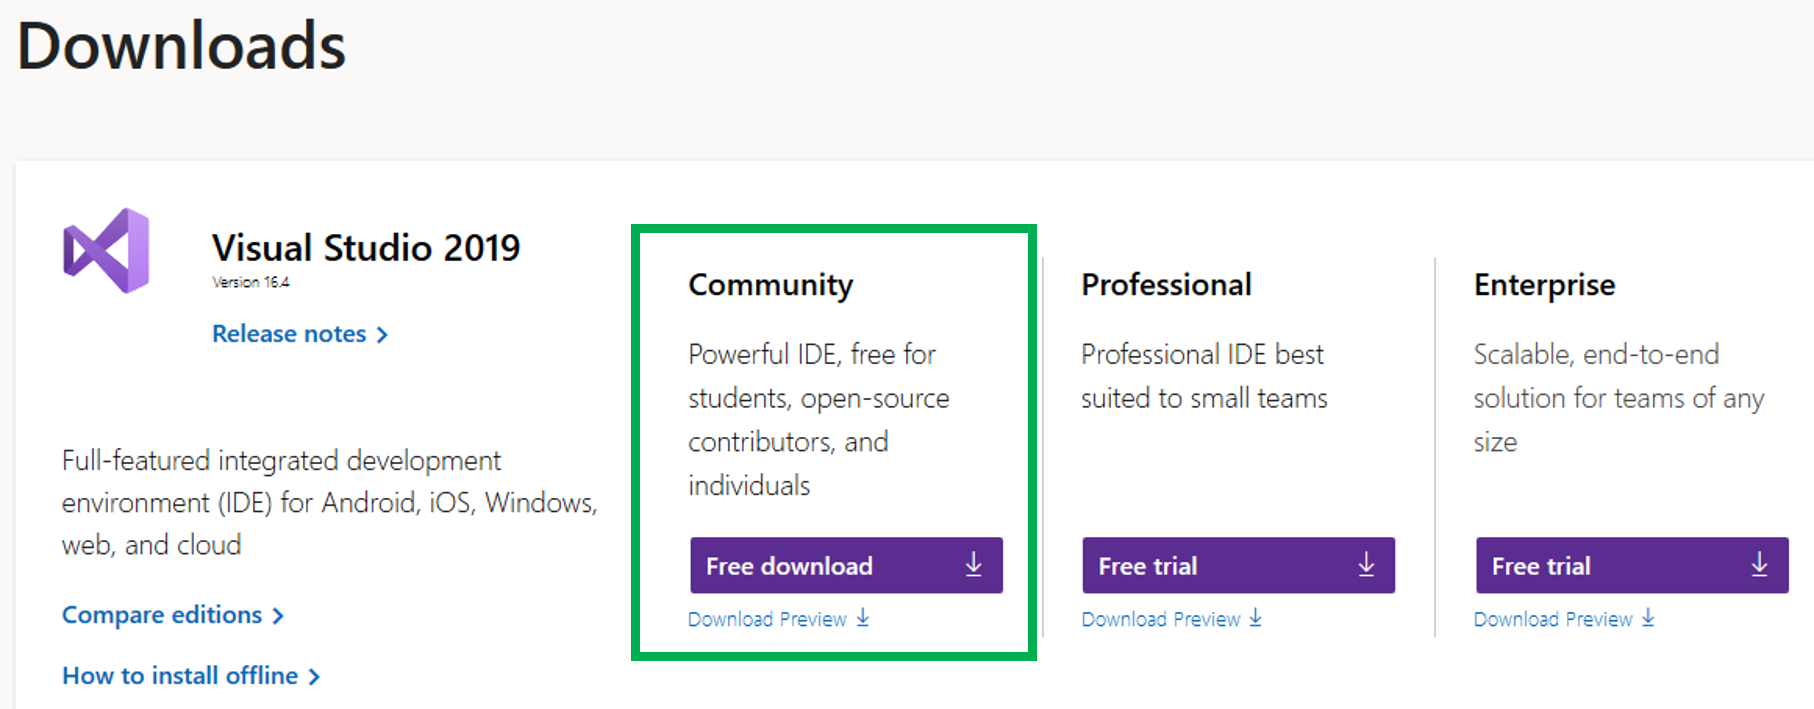
\includegraphics[width=0.9\linewidth]{images/auswahl_rahmenwerk/download.png}    
    \caption{Auswahl der Visual-Studio-Edition}
\end{figure}
Nach dem Download und anschließender Installation können die gewünschten Programmteile ausgewählt werden.
Für die Entwicklung von Xamarin-Applikationen ist das "Mobile development with .NET''-Paket erforderlich.


Keine weiteren Einstellungen oder Auswahlen sind zwingend erforderlich, allerdings empfiehlt es sich noch zusätzlich das ,,.NET desktop development''-Paket zu installieren.
Mit diesem kann man neue Technologien des .NET Frameworks in einer einfacheren Konsolenanwendung ausprobieren und kennenlernen.
\begin{figure}[H]
    \centering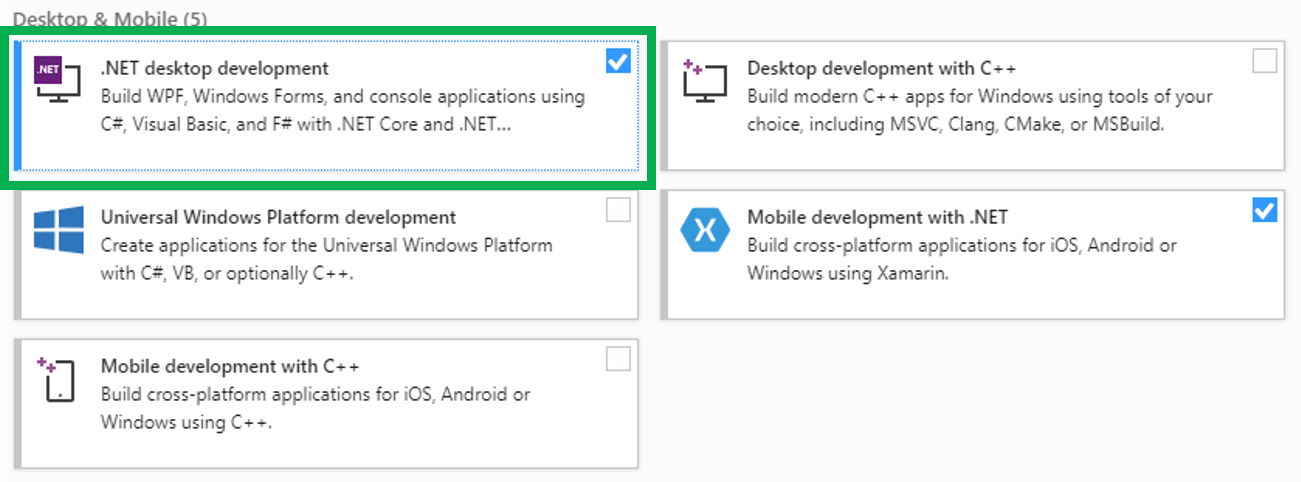
\includegraphics[width=0.9\linewidth]{images/auswahl_rahmenwerk/installation2.png}    
    \caption{Zusatzpaket für Desktop-Entwicklung mit .NET}
\end{figure}
Nach Fertigstellung der Installation von Visual Studio 2019 erscheint dieses am Desktop und im Startmenü als neues Icon.

\subsection{Installation Android SDK}
Das Xamarin-Rahmenwerk benötigt zum Entwickeln von Android-Apps noch zusätzlich mehrere Teile des Android SDK der Firma Google. Mit diesem wird während dem Kompilieren das Programm in ein installierbares Android-Paket, kurz APK, umgewandelt.
Damit dies richtig funktioniert, müssen alle Komponenten, auf die im Programm zugegriffen wird, über den Android-SDK-Manager installiert werden.
%Android SDK komponente
\begin{figure}[H]
    \centering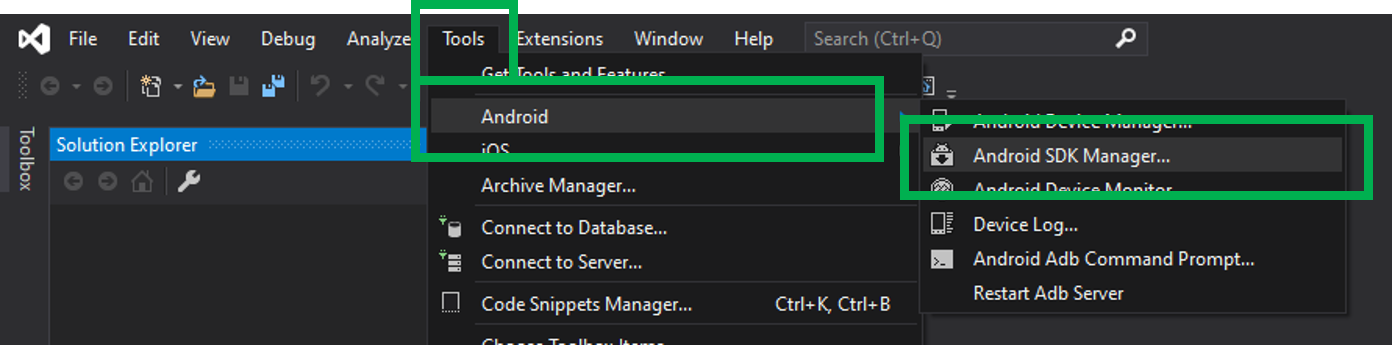
\includegraphics[width=0.9\linewidth]{images/auswahl_rahmenwerk/android_sdk_installation.png}    
    \caption{Android SDK Manager}
\end{figure}
\begin{figure}[H]
    \centering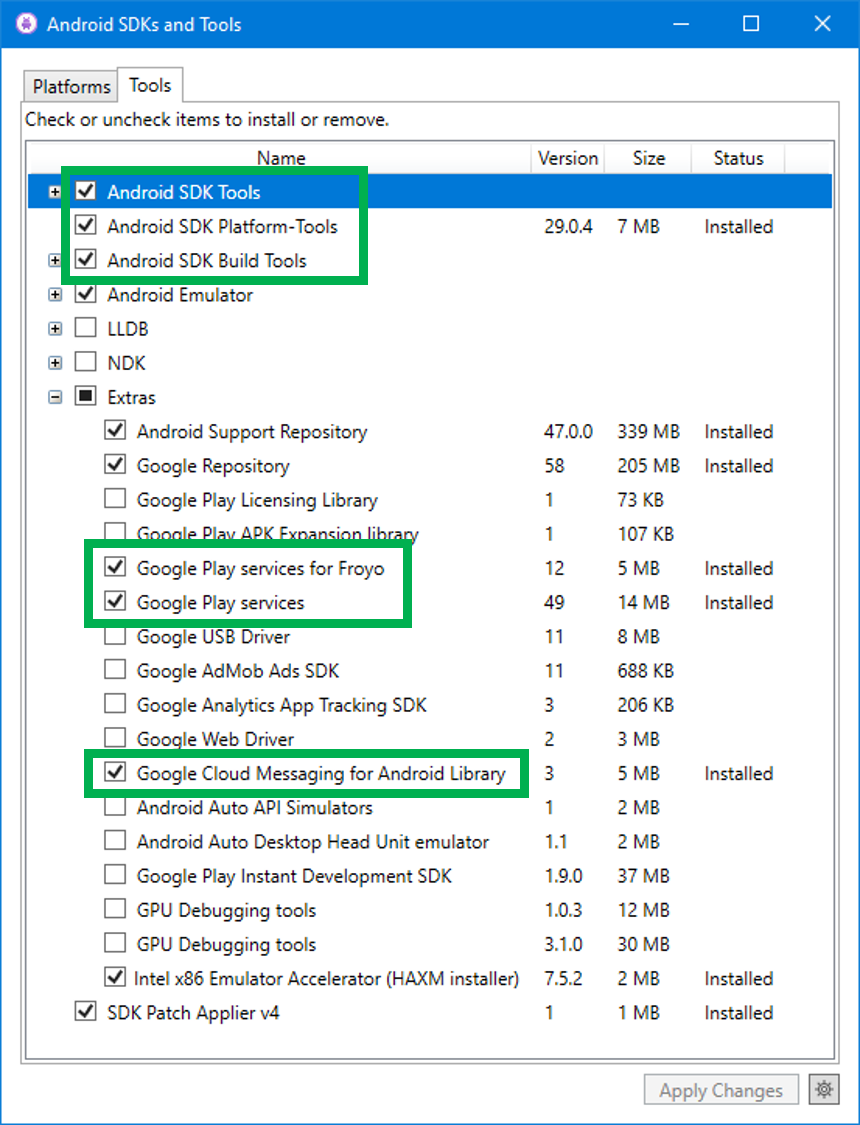
\includegraphics[height=15cm]{images/auswahl_rahmenwerk/android_sdk_auswahl.png}    
    \caption{Notwendige Teile des Android SDK}
\end{figure}
Besonders wichtig sind hier die Pakete der Google Play Services und die Google Cloud Messaging Library, welche für das Empfangen von Push-Benachrichtung zwingend erforderlich sind. Diese Benachrichtigung wird in einem eigenen Kapitel näher erklärt.
Die Android SDK Tools sind für jede Art von Android-Applikation mit Xamarin erforderlich.
Bei Bedarf kann über dieses Menü auch der offizielle Android-Emulator installiert werden.
%System images

Nach dem Start von Visual Studio muss eine neue ,,Solution'' angelegt werden. Diese beinhaltet alle Programmteile, welche für die Xamarin-Entwicklung benötigt werden. 

\begin{figure}[H]
    \centering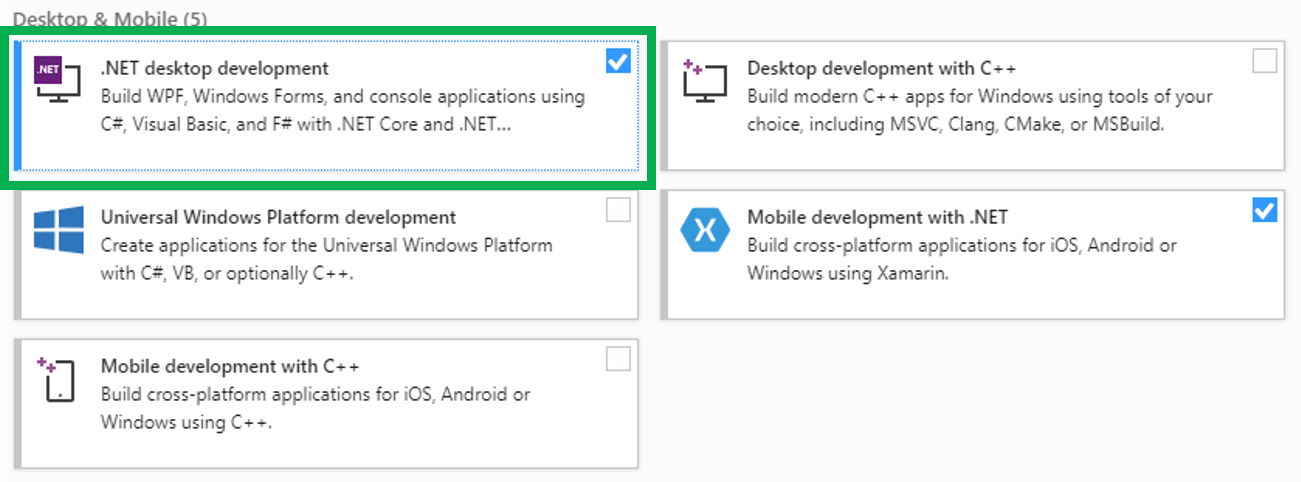
\includegraphics[width=0.9\linewidth]{images/auswahl_rahmenwerk/installation2.png}    
    \caption{Anlegen einer neuen Solution}
\end{figure}

%Weg vom Programm zur binary
%microsoft VS2019
%frei zugänglich
%nur auf windows, kein linux-support
%...